\begin{figure*}[h]
  \begin{center}
    \begin{tabular}{c}
      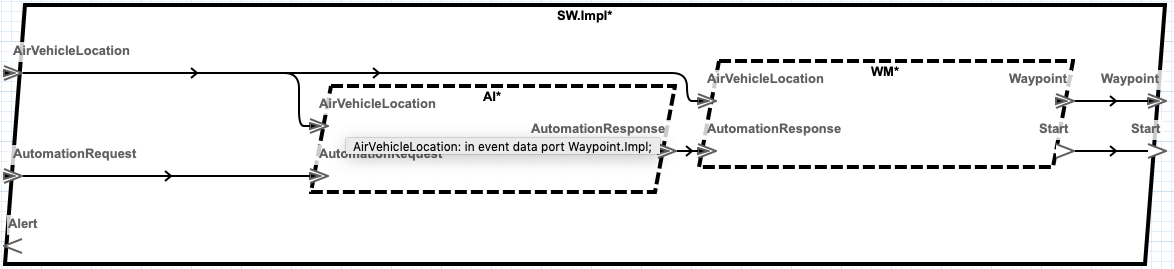
\includegraphics[scale=0.4]{example.png}
    \end{tabular}
  \end{center}
\caption{Initial design for an automated UAV route planning system.}
\label{fig:example}
\end{figure*}

\begin{figure}
  \begin{center}
    \begin{tabular}{c}
      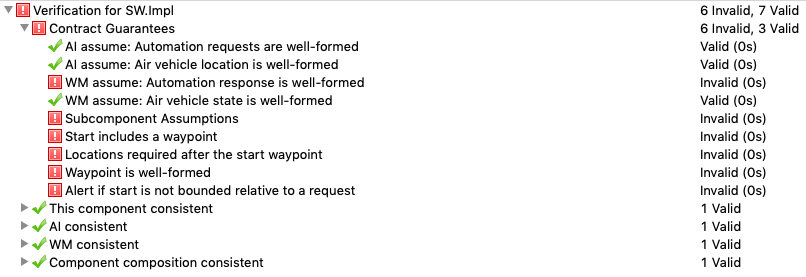
\includegraphics[scale=0.4]{example-certificate.png} \\
    \end{tabular}
  \end{center}
\caption{AGREE failure certificate for initial design.}
\label{fig:example-certificate}
\end{figure}

\figref{fig:example} is an AADL architectural model of a software
system (SW) for route planning and automated control of a UAV.  It is
loosely based on one of the case studies in
Section~\ref{sec:case-study}.  The source for the entire model is
found at \cite{repo}.

The system receives an automation request that is forwarded to a
third-party route planner (AI).  The route planner decides the flight
path of the UAV based on its current position and the requested task.
The waypoint manager (WM) receives the mission command as a set of
waypoints from the planner and starts the UAV flying the mission,
issuing waypoints to the UAV flight controller as the UAV location
changes.  The waypoint manager is a legacy component that cannot be
modified.

The expected behavior of the SW system, and the components
implementing the system, are modeled with AGREE contract
specifications.  The contracts constrain input with assumptions and
state properties of output with guarantees.  AGREE performs model
checking on this assume-guarantee system to hierarchically prove that
SW obeys all contract obligations under all possible finite input
streams.  The AGREE analysis, contract language, and contracts for SW
are discussed in greater detail in \secref{sec:agree}.

The initial AGREE contracts for the system in \figref{fig:example},
and its implementing components, both assume and guarantee the absence
of any malicious, or unspecified, component behavior.  More precisely,
the system contract assumes that all inputs are \emph{well-formed} and
there is never more than one automation request pending at a time.
The meaning of well-formed is given by user-written predicates for
each data type.  For example, a waypoint is well-formed if it falls
within bounds for latitude, longitude, and altitude.  The guarantees
for SW ensure that
\begin{itemize}
\item a start includes a waypoint,\footnote{KLS: maybe describe the start port earlier.}
\item a start is within one cycle of an automation request and if not, then it persistently alerts,
\item new waypoints coincide with air vehicle location updates, and
\item all outputs are well-formed.
\end{itemize}

The contracts for the sub-components assume their inputs are
well-formed, and they guarantee their outputs are well-formed.  The AI
contract guarantees it only responds to automation requests and always
in the same cycle.  The legacy WM contract guarantees the following: a
start from a response and always in the same cycle; start always comes
with a waypoint; and, further waypoints coincide with air vehicle
location updates.  These initial specifications pass AGREE
verification meaning that the contract composition of the components
with the system satisfies all component input assumptions and system
output guarantees.

\subsection{Detecting and addressing vulnerabilities}
A cyber-vulnerability analysis, however, identifies the potential of a
supply chain attack through the AI route planner (provided by a
third-party vendor without source code).  BriefCASE marks the
component as \emph{untrusted} after the analysis, and the contract for
AI is modified by removing all guarantees on its outputs to reflect
its untrusted status.  The AI output is now unconstrained in the
assume-guarantee reasoning of AGREE and is able to generate any value
on its output stream at anytime.

The output from the AGREE analysis using the untrusted AI
specification is shown in \figref{fig:example-certificate}.  The red
exclamation points designate component assumptions or system output
guarantees that do not hold, and each failure comes with a
corresponding counter-example.  The results are not unexpected given
the AI route planner's unconstrained behavior.

For example, the first violation is that the automation response from
the AI to the WM is no longer guaranteed to be well-formed.  The
consequence of that failing input assumption is that the WM outputs
are no longer guaranteed; they are effectively unconstrained.  These
missing output guarantees from the WM lead to the rest of the failures
in \figref{fig:example-certificate} because the WM provides the system
level outputs.

\begin{figure*}
  \begin{center}
    \begin{tabular}{c}
      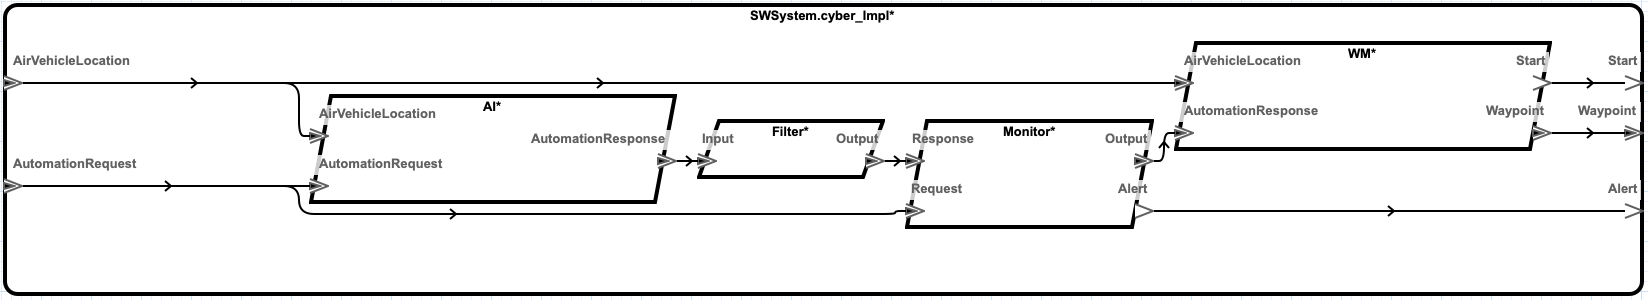
\includegraphics[scale=0.3]{hardened.png}
    \end{tabular}
  \end{center}
  \caption{Cyber-hardened design for an automated UAV route planning system}
  \label{fig:hardened}
\end{figure*}

\begin{figure}
  \begin{center}
    \begin{tabular}{c}
      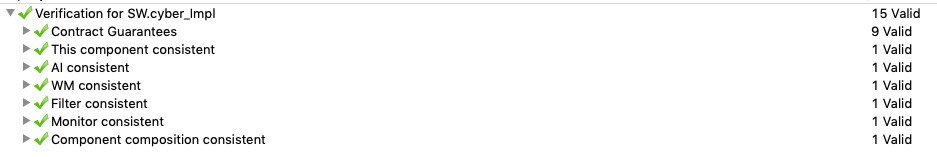
\includegraphics[scale=0.4]{hardened-certificate.png}
    \end{tabular}
  \end{center}
  \caption{AGREE verification certificate for cyber-hardened design.}
  \label{fig:hardened-certificate}
\end{figure}

The system designer now uses BriefCASE to cyber-harden SW by inserting
high-assurance components in the form of a filter and a monitor, as
shown in \figref{fig:hardened}.  A filter enforces an invariant over
each datum in the data stream by not forwarding input to its output if
that input violates the filter invariant.  The auto-generated AGREE
specification states that only well-formed inputs are passed to the
output.  The system developer must further define the filtering
policy, but it is usually based on the existing assumptions made by
downstream components that consume the filter output.

A monitor captures a relation on input data over time and is thus able
to reason about temporal properties of that input.  A monitor raises
an alert if the specified temporal properties are ever violated.  The
AGREE specification for the monitor in our example states that an
automation response can only be generated in conjunction with an
automation request; and further, that response must come with the
request or in the next step after the request.  As with the filter,
the system designer provides the policy, and that policy is typically
based on existing AADL/AGREE definitions in the SW system.

The AGREE analysis of the cyber-hardened implementation is shown in
\figref{fig:hardened-certificate}. AGREE has generated high-level
evidence justifying the claim that the high-assurance components
guarantee the correct behavior of the SW implementation in the
presence of the untrusted AI route planner.  Having passed AGREE
verification, the high-assurance components are ready to be
synthesized.

High-assurance components are automatically synthesized by SPLAT from
the AGREE specifications to equivalent programs in the CakeML
language.  The synthesis toolchain generates a proof that equates the
meaning of the AGREE specification to the behavior of the CakeML
program.  In other words, for any set of input streams that meet the
component's contract assumptions, the output streams produced from the
synthesized CakeML code exactly match those defined by the
high-assurance component's guarantees.  CakeML provides verified
compilation to binaries for several different platforms, meaning that
the resulting binaries exactly preserve the meaning of the original
CakeML code \cite{cakeml}.

Preserving the input to output relationship of streams between the
AGREE contracts and CakeML lifts the AGREE contract verification
results to the actual deployed system.  If the contract model
verification succeeds, then the meaning of those results hold for the
deployed system.  These results, however, are only valid under
additional assumptions on the deployed system:
\begin{itemize}
\item contracts for non-synthesized components accurately model their deployed
counterparts;
\item an appropriate schedule exists to sequence component
  execution following the dependent data-flow in the design; and
\item the communication fabric stitching components together works in harmony
  with the schedule.
\end{itemize}
\noindent Support and automation for these aspects of the design process are
discussed in other works.\footnote{KLS:need cites to HAMR, seL4, and Adventium work}
